\subsection*{Основные формулы}

Энергетическое разрешение спектрометра определяется, как
\begin{equation}
    R_i = \frac{\delta E_i}{E_i}, 
    \hspace{10 mm} 
    R_i = \frac{\const }{\sqrt{E_i}},
\end{equation}
где $\delta E_i$ -- ширина соответствующего максимума. 

Положение пика обратного рассеяния определяется по формуле 
\begin{equation}
    \sub{E}{обр} = \frac{E}{1 + 2 E/m c^2}
    ,
\end{equation}
где $E$ -- энергия соответствующего фотопика, $m c^2 = 511$ кэВ.

Максимальная энергия комптоновских электронов, соответствует 
\begin{equation*}
    \sub{E}{к, max} = \frac{\hbar \omega}{1 + m_e c^2 / 2 \hbar \omega}.
\end{equation*}


\subsection*{Экспериментальная установка}

\begin{figure}[h]
    \centering
    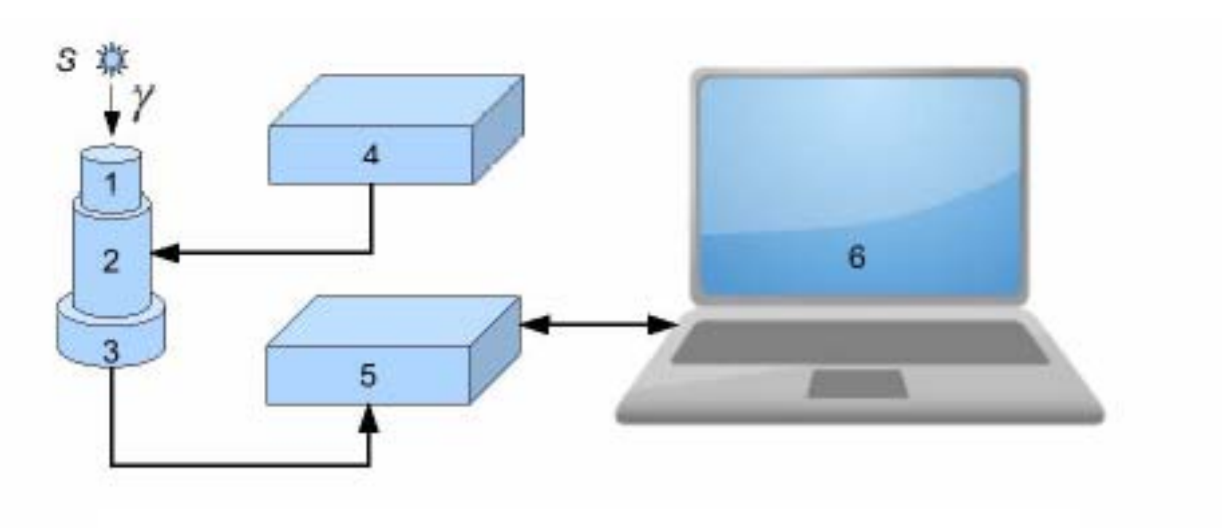
\includegraphics[width=0.4\textwidth]{figures/exp.png}
    \caption{Принципиальная блок-схема спектрометра}
    %\label{fig:}
\end{figure}
 На рисунке 1 -- сцинтиллятор, 2 -- ФЭУ, 3 -- предусилитель импульсов, 4 -- высоковольный блок питания для ФЭУ, 5 - АЦП, 6 -- компьютер для сбора даннных. 

 В качестве сцинтиллятора  используютсся кристаллы NaI(Tl). 

 Излучение образца улавливается сцинтиллятором, затем, с помощью ФЭУ, и описанной схемы преобразуется в спектрограмму.



\newpage

